% =====================================================================
% NeuroPulse -- Camera-Ready Copy (Springer LNCS/LNNS / llncs)
% Compile: pdflatex main.tex; bibtex main; pdflatex main.tex; pdflatex main.tex
% =====================================================================
\documentclass[a4paper,runningheads,orivec]{llncs}

\usepackage[T1]{fontenc}
\usepackage{amsmath}
\usepackage{newtxtext}
\usepackage[varvw]{newtxmath}
\usepackage{graphicx}
\usepackage{booktabs}
\usepackage{microtype}
\usepackage{tikz}
\usepackage{url}
\usepackage{bbding}
\providecommand{\Description}[1]{}

% ---- notation shortcuts ------------------------------------------------
\newcommand{\R}{\mathbb{R}}
\newcommand{\bx}{\mathbf{x}}
\newcommand{\bz}{\mathbf{z}}
\newcommand{\bh}{\mathbf{h}}
\newcommand{\bw}{\mathbf{w}}
\newcommand{\bp}{\mathbf{p}}
\newcommand{\bF}{\mathbf{F}}
\newcommand{\Tcal}{T_{\mathrm{cal}}}
\DeclareMathOperator{\sigm}{sigmoid}
\DeclareMathOperator{\logit}{logit}
\DeclareMathOperator{\clip}{clip}
\DeclareMathOperator{\softmax}{softmax}
\DeclareMathOperator{\Var}{Var}
\DeclareMathOperator*{\argmax}{arg\,max}

\begin{document}

\title{NeuroPulse: Orthogonal Four-Stream Deepfake Video Detection via Haemodynamic Signal Analysis, Depthwise-Separable Spatio-Temporal Dual-Branch Attention, and Hierarchical Shifted-Window Transformer Late-Fusion Ensemble}
\titlerunning{NeuroPulse: Four-Stream Deepfake Detection}

\author{\mbox{Vasireddy Likhith Chowdary}\orcidID{0009-0000-5291-8452}~(\Envelope) \and
\mbox{Raushan Kumar Singh} \and
\mbox{Lalith Sathvik Gaddam} \and
\mbox{Dheeraj Thirunala} \and
\mbox{Siva Nikshya Vishnumolakala} \and
\mbox{Katta Tejaswi}}

\authorrunning{V. L. Chowdary et al.}

\institute{Department of Computer Science and Engineering, SRM University-AP, Amaravati 522240, Andhra Pradesh, India\\
\email{\{likhithchowdary\_vasireddy,\allowbreak{}raushankumar.s,\allowbreak{}lalithsathvik\_gaddam,\allowbreak{}dheeraj\_thirunala,\allowbreak{}sivanikshya\_vishnumolakala,\allowbreak{}tejaswi\_katta\}@srmap.edu.in}}

\maketitle

\begin{abstract}
Single-cue deepfake detectors often degrade when synthesis suppresses spatial artefacts or enforces temporal smoothing, while subject overlap across splits can inflate benchmark metrics. We present NeuroPulse, a four-stream forensic framework capturing complementary biological, spatial, temporal, and spectral manipulation traces. Stream~I extracts a 117-dimensional, nine-region CHROM-rPPG haemodynamic descriptor for gradient-boosted stacking. Stream~II couples EfficientNet-B4 with a bidirectional LSTM and multi-head temporal attention. Stream~III integrates depthwise-separable Xception convolutions, Efficient Channel Attention (ECA), a parallel learned-feature branch, and online hard-example mining. Stream~IV combines a hierarchical Swin-Tiny transformer with an analytic block-DCT frequency branch and a packed-sequence BiLSTM. Late fusion unifies Bayesian-ridge iterative imputation, out-of-fold beta calibration, multi-objective NSGA-II Pareto weight search, temperature scaling, and split-conformal prediction. On a balanced 1,754-video corpus spanning 1,042 identity-disjoint groups, our Pareto-optimal ensemble fuses the rPPG, EfficientNet-B4, and Swin-Tiny streams to reach 0.8081 AUC (95\% CI: 0.7856--0.8293), 72.9\% accuracy, and 0.734 F1, outperforming all single streams. Low rPPG--Swin correlation ($r{=}0.232$) confirms cross-modal synergy, with 90.07\% conformal coverage at $\alpha{=}0.1$.
\keywords{Deepfake detection \and Remote photoplethysmography \and Swin Transformer \and Efficient Channel Attention \and DCT frequency analysis \and Calibrated late fusion}
\end{abstract}

% =====================================================================
\section{Introduction}
GANs~\cite{goodfellow2014gan}, face-swapping pipelines, and diffusion models~\cite{ho2020ddpm} synthesise high-fidelity portrait videos that pose severe risks of disinformation, identity fraud, and non-consensual media~\cite{li2020celebdf,rossler2019ff}. Relying on a single forensic modality creates vulnerability: compression attenuates spatial artefacts, whereas generators smooth frame transitions yet struggle to maintain coherent physiological blood-volume pulsations~\cite{ciftci2020fakecatcher}. Moreover, subject overlap between splits can reward identity memorisation over forgery detection.

NeuroPulse addresses these challenges through four architecturally distinct forensic pathways: haemodynamic biosignal analysis, compound-scaled convolutional spatio-temporal modelling, dual-branch depthwise-separable attention, and hierarchical shifted-window transformer/DCT spectral analysis. Here, ``orthogonal'' denotes architectural separation across complementary physical and computational mechanisms. Contributions are: (1)~a four-stream forensic framework exploiting complementary failure modes; (2)~a nine-region, 117-feature CHROM-rPPG descriptor with two-level stacking; (3)~EfficientNet-B4, Xception, and Swin-Tiny streams with BiLSTM/attention, ECA, MixUp/CutMix, hard-example mining, and a frame curriculum; (4)~calibrated late fusion uniting iterative imputation, beta calibration, NSGA-II Pareto weighting, temperature scaling, and conformal prediction; and (5)~identity-disjoint group evaluation across 1,042 subjects.

\section{Related Work}
FaceForensics++~\cite{chollet2017xception,rossler2019ff}, Celeb-DF~\cite{li2020celebdf}, and DFDC~\cite{dolhansky2020dfdc} support evaluation across diverse synthesis methods and compression levels, while frequency analyses~\cite{frank2020leveraging} show that upsampling leaves spectral periodicities. EfficientNet~\cite{tan2019efficientnet}, Swin~\cite{liu2021swin}, and ECA-Net~\cite{wang2020eca} motivate our visual streams. FakeCatcher~\cite{ciftci2020fakecatcher}, DeepRhythm~\cite{qi2020deeprhythm}, CHROM~\cite{dehaan2013chrom}, and POS~\cite{wang2017pos} motivate physiological cues, while calibration~\cite{guo2017calibration,kull2017beta} and conformal prediction~\cite{vovk2005conformal} ensure score reliability within our unified ensemble.

% =====================================================================
\section{Framework, Data, and Pre-Processing}
\subsection{Four-Stream Architecture and Complementarity}
NeuroPulse exploits complementary failure modes: compression may erase spatial seams while leaving haemodynamic phase incoherence intact, whereas high-fidelity rendering may evade spatial detectors but disrupt cardiac pulse synchronisation or block-DCT spectra. Each stream $i\in\{1,\dots,4\}$ emits a fake probability $p_i\in[0,1]$ for late fusion (Fig.~\ref{fig:overview}).

\begin{figure}[!t]
\centering
\resizebox{\linewidth}{!}{%
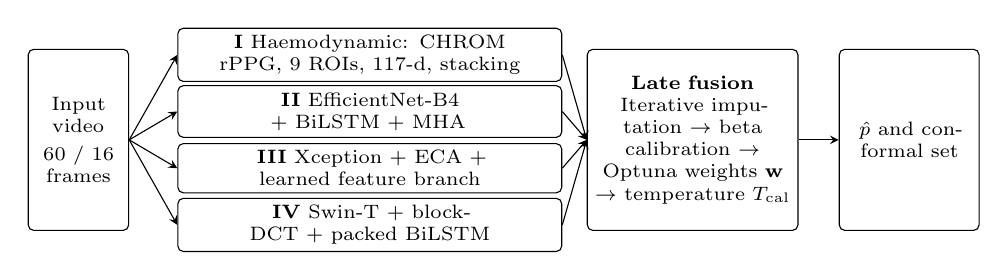
\begin{tikzpicture}[x=1cm,y=1cm,
b/.style={draw,rounded corners=2pt,align=center,font=\scriptsize,inner sep=2.5pt},
a/.style={-stealth,thin}]
\node[b,minimum height=2.3cm,text width=1.1cm] (in) at (0.75,0) {Input video\\[2pt] 60 / 16 frames};
\node[b,text width=4.7cm] (s1) at (4.45,1.08) {\textbf{I}~Haemodynamic: CHROM rPPG, 9 ROIs, 117-d, stacking};
\node[b,text width=4.7cm] (s2) at (4.45,0.36) {\textbf{II}~EfficientNet-B4 + BiLSTM + MHA};
\node[b,text width=4.7cm] (s3) at (4.45,-0.36) {\textbf{III}~Xception + ECA + learned feature branch};
\node[b,text width=4.7cm] (s4) at (4.45,-1.08) {\textbf{IV}~Swin-T + block-DCT + packed BiLSTM};
\node[b,minimum height=2.3cm,text width=2.5cm] (f) at (8.55,0) {\textbf{Late fusion}\\Iterative imputation $\to$ beta calibration $\to$ Optuna weights $\bw$ $\to$ temperature $\Tcal$};
\node[b,minimum height=2.3cm,text width=1.6cm] (o) at (11.3,0) {$\hat p$ and conformal set};
\foreach \s in {s1,s2,s3,s4}{\draw[a] (in.east)--(\s.west); \draw[a] (\s.east)--(f.west);}
\draw[a] (f.east)--(o.west);
\end{tikzpicture}%
}
\Description{Flow diagram: one video input feeds CHROM-rPPG; EfficientNet-B4 with BiLSTM and multi-head attention; Xception with ECA and a learned-feature branch; and Swin-Tiny with block-DCT and a packed BiLSTM. Their scores feed late fusion and a conformal-prediction output.}
\caption{NeuroPulse architecture showing four complementary streams, calibrated late fusion, and uncertainty-aware prediction.}
\label{fig:overview}
\end{figure}

\subsection{Corpus and Identity-Disjoint Evaluation}
The corpus integrates FaceForensics++~\cite{rossler2019ff} (C23 originals and six manipulation subsets, up to 200 each), Celeb-DF\,v2~\cite{li2020celebdf} (150+50 real, 200 synthesised), a DFDC sample~\cite{dolhansky2020dfdc}, and a custom 400+400 collection. Class balancing, $n_{\mathrm{balanced}}=\min(|\mathcal R|,|\mathcal F|)$, yields 877 real and 877 fake videos (1,754 total) across 1,042 subject-identity labels. Dataset-specific identity keys drive stratified group $K$-fold ($K{=}5$) partitioning, enforcing for each fold $q$:
\begin{equation}
\bigl(\mathrm{ID}^{(q)}_{\mathrm{train}}\cap \mathrm{ID}^{(q)}_{\mathrm{val}}\bigr)=\emptyset ,
\label{eq:leak}
\end{equation}
verified by assertion before every run, with thresholds tuned on validation data only to guarantee zero subject-identity leakage between splits.

\subsection{Face Localisation, Alignment, and Quality Control}
Stream~I uses MediaPipe FaceMesh~\cite{kartynnik2019facemesh} (468 landmarks) on up to 60 uniformly sampled frames; Streams~II--IV use MTCNN~\cite{zhang2016mtcnn} on $T{=}16$ uniform frames, with a centre-crop fallback. For Streams~III--IV, eye landmarks define roll $\theta=\operatorname{arctan2}(\Delta y_{\mathrm{eyes}},\Delta x_{\mathrm{eyes}})$, de-rotating crops when $|\theta|>2^{\circ}$. Crops with Laplacian variance $\Var[\nabla^{2}I]<20.0$ are rejected as blurry.

% =====================================================================
\section{Stream I: Haemodynamic rPPG Analysis}
Cardiac blood-volume pulses produce subtle skin-reflectance fluctuations (rPPG). NeuroPulse targets four physiological cues: (1)~\emph{spatial coherence}, as the arterial pulse wave (5--10\,m/s) reaches facial regions with anatomical phase delays that synthesis disrupts; (2)~\emph{spectral concentration} in the 0.7--4.0\,Hz band; (3)~\emph{heart-rate variability (HRV) dynamics}; and (4)~\emph{cross-region phase-locking synchronisation}~\cite{lachaux1999plv}.

Nine convex-hull regions (forehead centre, left/right forehead, cheeks, nose, chin, and jaws) provide high capillary density and bilateral symmetry. For region mask $\Omega_r$ in frame $t$, mean RGB colour is extracted and CHROM~\cite{dehaan2013chrom} projects reflected light into chrominance channels to suppress specular noise:
\begin{align}
\bar{\mathbf c}^{(r)}_t&=\frac{1}{|\Omega_r|}\sum_{(x,y)\in\Omega_r}\mathbf I_t(x,y),\\
X_{\mathrm{CHROM}}&=3R-2G,\qquad Y_{\mathrm{CHROM}}=1.5R+G-1.5B,\\
\mathrm{BVP}(t)&=X_{\mathrm{CHROM}}(t)-\frac{\sigma_X}{\sigma_Y}\,Y_{\mathrm{CHROM}}(t),
\end{align}
where $R,G,B$ are ROI-averaged channels and $\sigma_X,\sigma_Y$ are sliding-window standard deviations. Using mean-normalised signals $R_n,G_n,B_n$, the windowed extractor computes:
\begin{align}
X_s&=3R_n-2G_n,\qquad Y_s=1.5R_n+G_n-1.5B_n,\\
\alpha_c&=\clip\!\Bigl(\tfrac{\sigma(X_s)}{\sigma(Y_s)},\,0,\,10\Bigr),\qquad P=X_s-\alpha_c Y_s.
\end{align}
Window length is $w=\max(\lfloor 1.6\,f_s\rfloor,2)$ and step $s=\max(1,\lfloor w/2\rfloor)$ (50\% overlap). After overlap-add reconstruction, the signal is detrended and filtered via a 3rd-order Butterworth band-pass filter~\cite{butterworth1930}:
\begin{equation}
\lvert H(\mathrm{j}\omega)\rvert^{2}=\Bigl[1+\Bigl(\frac{\omega^{2}-\omega_L\omega_H}{(\omega_H-\omega_L)\,\omega}\Bigr)^{2n}\Bigr]^{-1},\qquad n=3.
\end{equation}
Cutoffs are $f_L{=}0.7$\,Hz and $f_H{=}4.0$\,Hz (42--240\,BPM). Gaps under 30\% of frames are linearly interpolated, POS~\cite{wang2017pos} is the fallback, and spectra use Welch's method~\cite{welch1967} ($n_{\mathrm{perseg}}{=}\min(256,\lfloor T/2\rfloor)$, $n_{\mathrm{fft}}{=}1024$).

The 117-dimensional descriptor spans \textbf{spectral} features (24: SNR, purity, prominence, dominant frequency, harmonic ratio, entropy, centroid, and temporal moments); \textbf{HRV and phase} (13: eight HRV metrics including RMSSD, SDNN, pNN50, and LF/HF, plus five Hilbert phase/BPM features); \textbf{cross-ROI coherence} (18); \textbf{geometry} (26 scale-invariant landmark ratios); and \textbf{signal quality/multi-band energy} (36). Phase synchronisation across region pairs is quantified via the Phase Locking Value~\cite{lachaux1999plv}:
\begin{equation}
\mathrm{PLV}_{ab}=\left|\frac{1}{N}\sum_{t=1}^{N}e^{\,\mathrm{j}(\phi_a(t)-\phi_b(t))}\right|,
\end{equation}
where $\mathrm{j}^{2}=-1$ and $\phi_a(t)$ is the instantaneous Hilbert phase. After percentile clipping, median imputation, scaling, and ExtraTrees selection, XGBoost~\cite{chen2016xgboost} (300 trees), LightGBM~\cite{ke2017lightgbm} (8 leaves), and HistGradientBoosting (300 iterations) feed an $\ell_2$ logistic-regression meta-learner via 5-fold stacked generalisation~\cite{wolpert1992stacking}.

% =====================================================================
\section{Stream II: EfficientNet-B4 Spatio-Temporal Network}
EfficientNet-B4~\cite{tan2019efficientnet} (stochastic-depth rate 0.2; global average pooling) maps each frame $\bx_{b,t}$ to:
\begin{equation}
\mathbf f_{b,t}=\text{EfficientNet-B4}(\bx_{b,t})\in\R^{1792}.
\end{equation}
Omitting batch index $b$, a 2-layer bidirectional LSTM~\cite{hochreiter1997lstm} models temporal transitions (256 hidden units per direction; inter-layer dropout 0.5):
\begin{align}
\overrightarrow{\bh}_t&=\mathrm{LSTM}_{\mathrm{fwd}}(\mathbf f_t,\overrightarrow{\bh}_{t-1}),\quad
\overleftarrow{\bh}_t=\mathrm{LSTM}_{\mathrm{bwd}}(\mathbf f_t,\overleftarrow{\bh}_{t+1}),\\
\bh_t&=[\overrightarrow{\bh}_t;\overleftarrow{\bh}_t]\in\R^{512}.
\end{align}
A 4-head self-attention layer~\cite{vaswani2017attention} with key-padding masks enables global cross-frame interaction. Residual LayerNorm outputs $\mathbf a_t$ and validity masks $m_t\in\{0,1\}$ feed masked average pooling to form the 512-d video descriptor:
\begin{align}
\mathrm{head}_h&=\softmax\!\left(\frac{\mathbf Q\mathbf W^{Q}_h(\mathbf K\mathbf W^{K}_h)^{\top}}{\sqrt{d_k}}\right)\mathbf V\mathbf W^{V}_h,\\
\mathrm{MHA}&=[\mathrm{head}_1;\dots;\mathrm{head}_4]\,\mathbf W^{O},\qquad
\bz=\frac{\sum_{t=1}^{T}m_t\,\mathbf a_t}{\sum_{t=1}^{T}m_t}.
\end{align}
A LayerNorm/GELU MLP head (512$\to$256$\to$128$\to$1; dropout 0.5, 0.25) maps $\bz$ to logit $\hat y$. Focal loss~\cite{lin2017focal} uses $\alpha{=}0.6$, $\gamma{=}2.0$, and label smoothing $\epsilon{=}0.1$. For hard label $y\in\{0,1\}$, $p=\sigm(\hat y)$, $y_\epsilon=y(1-\epsilon)+0.5\epsilon$, and $p_t^{\mathrm{clip}}=\clip(p_t,10^{-7},1-10^{-7})$, the per-sample loss is:
\begin{align}
p_t&=py+(1-p)(1-y),\quad \alpha_t=\alpha y+(1-\alpha)(1-y),\\
\mathcal L_{\mathrm{FL}}(\hat y,y)&=-\alpha_t(1-p_t^{\mathrm{clip}})^\gamma\bigl[y_\epsilon\log p+(1-y_\epsilon)\log(1-p)\bigr].
\end{align}
Sequence-level MixUp~\cite{zhang2018mixup} is applied with probability 0.3 per batch using cyclic non-identity pairing ($\lambda\sim\mathrm{Beta}(1.0,1.0)$), evaluating the focal criterion on both hard targets:
\begin{align}
\tilde{\bx}&=\lambda\bx_i+(1-\lambda)\bx_j,\quad \tilde y=\lambda y_i+(1-\lambda)y_j,\\
\mathcal L_{\mathrm{mix}}&=\lambda\,\mathcal L_{\mathrm{FL}}(\hat y,y_i)+(1-\lambda)\,\mathcal L_{\mathrm{FL}}(\hat y,y_j).
\end{align}
Stochastic weight averaging (SWA)~\cite{izmailov2018swa} from epoch 30 maintains the running mean:
\begin{equation}
\bar{\boldsymbol\theta}_n=\frac{n-1}{n}\,\bar{\boldsymbol\theta}_{n-1}+\frac{1}{n}\,\boldsymbol\theta_n ,
\end{equation}
with the backbone learning rate at $0.1\times$ base. Inference averages five TTA passes; gradient accumulation over four micro-batches of two videos gives an effective batch of 8. Figure~\ref{fig:eff} shows the training/evaluation curves, and Fig.~\ref{fig:gradcam} visualises Grad-CAM~\cite{selvaraju2017gradcam} attention on blending boundaries.

\begin{figure}[!t]
\centering
\begin{minipage}[t]{0.495\textwidth}
\centering
\includegraphics[width=\linewidth]{EFFICIENTNET_training_curves.png}
\par\smallskip
{\small (a) Training}
\end{minipage}\hfill
\begin{minipage}[t]{0.495\textwidth}
\centering
\includegraphics[width=\linewidth]{EFFICIENTNET_evaluation_plots.png}
\par\smallskip
{\small (b) Evaluation}
\end{minipage}
\Description{The training panel shows loss, AUC, validation F1, precision, recall, and the learning-rate schedule over epochs. The evaluation panel shows a ROC curve, precision-recall curve, confusion matrix, and score distributions for the EfficientNet-B4 classifier.}
\caption{EfficientNet-B4 training (a) and evaluation (b). SWA begins at epoch 30; validation AUC stabilises near 0.739 at epoch 31.}
\label{fig:eff}
\end{figure}

\begin{figure}[!t]
\centering
\includegraphics[width=\linewidth,height=3.1cm,keepaspectratio]{EFFICIENTNET_gradcam_gallery.png}
\Description{A gallery of Grad-CAM visualisations for three illustrative validation videos. Each row shows frames with coloured activation heatmaps overlaid on faces, highlighting periorbital, nasal, and mouth blending boundaries.}
\caption{Grad-CAM~\cite{selvaraju2017gradcam} activation maps (\texttt{conv\_head}) across three validation videos, illustrating spatial attention on facial blending seams and ocular/oral regions.}
\label{fig:gradcam}
\end{figure}

% =====================================================================
\section{Stream III: Depthwise-Separable Xception Dual-Branch Network}
Xception~\cite{chollet2017xception} factorises convolution into depthwise filtering and pointwise $1{\times}1$ mixing to isolate boundary seam and texture artefacts, yielding 2048-d frame features at $299{\times}299$. ECA-Net~\cite{wang2020eca} recalibrates channels via a 1D convolution of adaptive kernel size ($k{=}7$ for $C{=}2048$):
\begin{align}
k&=\mathrm{odd}\!\left(\left\lceil\frac{\log_2 C+1}{2}\right\rceil\right),\\
\mathbf g&=\sigm\!\bigl(\mathrm{Conv1d}_k(\mathrm{GAP}(\bF))\bigr),\qquad \hat{\bF}=\mathbf g\odot\bF .
\end{align}
A \emph{parallel learned-feature branch} projects global-pooled ECA features into a 256-d auxiliary embedding $\bz_{\mathrm{aux}}$ and concatenates it with the 512-d BiLSTM--MHA temporal representation:
\begin{align}
\bz_{\mathrm{aux}}&=\mathrm{LN}\bigl(\mathrm{Linear}_{256}(\mathrm{GELU}(\mathrm{LN}(\mathrm{Linear}_{256}(\mathrm{GAP}(\hat{\bF}))))) \bigr)\in\R^{256},\\
\bz_{\mathrm{fused}}&=[\bz_{\mathrm{temporal}};\,\bz_{\mathrm{aux}}]\in\R^{768}.
\end{align}
An MLP head (768$\to$256$\to$128$\to$1; dropout 0.3, 0.15) scores $\bz_{\mathrm{fused}}$. From epoch 10, online hard-example mining~\cite{shrivastava2016ohem} scores boundary proximity and refreshes a class-balanced sampler every 5 epochs to up-sample ambiguous videos ($h_i\approx1$):
\begin{align}
\alpha_{\mathrm{fold}}&=\frac{N_{\mathrm{real}}}{N_{\mathrm{real}}+N_{\mathrm{fake}}},\\
h_i&=1-2\,|p_i-0.5|.
\end{align}
With probability 0.3, MixUp ($\alpha{=}0.2$) or CutMix~\cite{yun2019cutmix} ($\alpha{=}1.0$) is selected equally often. CutMix splices facial patches across sequences to simulate blending seams:
\begin{equation}
\tilde{\bx}=\mathbf M\odot\bx_i+(1-\mathbf M)\odot\bx_j,\qquad \lambda_{\mathrm{adj}}=\frac{\|\mathbf M\|_1}{HW}.
\end{equation}
The mixed label is $\tilde y=\lambda_{\mathrm{adj}}y_i+(1-\lambda_{\mathrm{adj}})y_j$; Fig.~\ref{fig:xcep} shows Stream~III reaching 0.785 AUC.

\begin{figure}[!t]
\centering
\begin{minipage}[t]{0.495\textwidth}
\centering
\includegraphics[width=\linewidth]{XCEPTION_training_curves.png}
\par\smallskip
{\small (a) Training}
\end{minipage}\hfill
\begin{minipage}[t]{0.495\textwidth}
\centering
\includegraphics[width=\linewidth]{XCEPTION_evaluation_plots.png}
\par\smallskip
{\small (b) Evaluation}
\end{minipage}
\Description{The training panel shows loss, training and validation AUC, validation F1, precision, recall, and the learning-rate schedule over epochs. The evaluation panel shows ROC and precision-recall curves, a confusion matrix, and predicted-score distributions for Xception.}
\caption{Xception training (a) and evaluation (b). Hard-example mining starts at epoch 10 and SWA at epoch 15, reaching a validation AUC of 0.785 and AP of 0.760.}
\label{fig:xcep}
\end{figure}

% =====================================================================
\section{Stream IV: Hierarchical Swin Transformer with DCT Branch}
Swin-Tiny~\cite{liu2021swin} (patch size 4, $M{=}7$ windows) applies self-attention within non-overlapping $M{\times}M$ windows---reducing complexity from $O(N^2)$ to $O(NM^2)$---while alternating shifted windows to capture cross-boundary seams across $\tfrac H4{\times}\tfrac W4$, $\tfrac H8{\times}\tfrac W8$, $\tfrac H{16}{\times}\tfrac W{16}$, and $\tfrac H{32}{\times}\tfrac W{32}$ scales:
\begin{equation}
\text{W-MSA}(\mathbf Q,\mathbf K,\mathbf V)=\softmax\!\left(\frac{\mathbf Q\mathbf K^{\top}}{\sqrt d}+B\right)\mathbf V,
\end{equation}
with learnable relative position bias $B$. To prevent padding from skewing normalisation statistics, padded frames bypass the backbone:
\begin{equation}
\mathbf s_t=\begin{cases}\mathrm{Swin}(\bx_t)&m_t=1,\\ \mathbf 0&m_t=0.\end{cases}
\end{equation}
The 768-d output is recalibrated by a fixed-kernel ($k{=}5$) ECA layer and projected to 384-d.

\subsubsection{On-the-Fly DCT Spectral Branch.} To capture upsampling and generator periodicities directly from pixels, a precomputed orthonormal 2D DCT-II basis~\cite{ahmed1974dct} transforms each down-sampled $64{\times}64$ luminance crop ($N{=}64$, $\alpha_0{=}\sqrt{1/N}$, $\alpha_k{=}\sqrt{2/N}$ for $k>0$):
\begin{align}
D_{k,n}&=\alpha_k\cos\!\left(\frac{\pi k(2n+1)}{2N}\right),\quad k,n\in\{0,\dots,N{-}1\},\\
\mathbf X_{\mathrm{DCT}}&=\mathbf D\,\mathbf I_{\mathrm{gray}}\,\mathbf D^{\top},\quad I_{\mathrm{gray}}=0.299\,R+0.587\,G+0.114\,B.
\end{align}
Log-magnitude coefficients, $\hat X_{k,l}=\log(|X_{k,l}|+10^{-6})$, are partitioned into 64 non-overlapping $8{\times}8$ sub-bands whose means $\mu_b$ and standard deviations $\sigma_b$ form:
\begin{equation}
\mathbf f_{\mathrm{DCT}}=[\mu_1,\sigma_1,\mu_2,\sigma_2,\ldots,\mu_{64},\sigma_{64}]\in\R^{128}.
\end{equation}
A two-layer MLP encodes $\mathbf f_{\mathrm{DCT}}$ into $\bz_{\mathrm{freq}}^{192}$. Packed sequences keep padding out of the 2-layer BiLSTM (input 384, hidden 256; Xavier-uniform input, orthogonal recurrent weights, forget-gate bias initialised to 1.0). For sample $b$ in a minibatch of $N_B$ videos, valid length $\ell_b$ and the 704-d fused representation are:
\begin{align}
\ell_b&=\sum_{t=1}^{T}m_{b,t},\qquad\forall b\in\{1,\dots,N_B\},\\
\bz&=[\bz_{\mathrm{temporal}}^{512};\,\bz_{\mathrm{freq}}^{192}]\in\R^{704},
\end{align}
followed by 4-head attention and an MLP head (704$\to$192$\to$96$\to$1). Training follows a progressive frame curriculum (validation always uses 16 frames):
\begin{equation}
T_{\mathrm{train}}(e)=\begin{cases}5&e\in[0,4],\\10&e\in[5,14],\\16&e\ge15.\end{cases}
\end{equation}
Across all five identity-disjoint folds, Stream~IV achieves per-fold best AUCs of 0.762, 0.836, 0.802, 0.781, and 0.776 (mean $0.791\pm0.026$) and a pooled out-of-fold (OOF) AUC of 0.789 (95\% CI: 0.768--0.810) over 1,753 videos (Fig.~\ref{fig:swin}).

\begin{figure}[!t]
\centering
\begin{minipage}[t]{0.495\textwidth}
\centering
\includegraphics[width=\linewidth]{SWIN_training_curves.png}
\par\smallskip
{\small (a) Training}
\end{minipage}\hfill
\begin{minipage}[t]{0.495\textwidth}
\centering
\includegraphics[width=\linewidth]{SWIN_evaluation_plots.png}
\par\smallskip
{\small (b) Evaluation}
\end{minipage}
\Description{The training panel shows the selected Swin-Tiny fold (Fold 1) with loss, training and validation AUC, training phases, and learning-rate schedule over epochs. The evaluation panel shows Fold 1 post-hoc ROC and precision-recall curves, a confusion matrix, and predicted-score distributions.}
\caption{Swin-Tiny curriculum training on Fold 1 (a, 0.836 AUC) and post-hoc evaluation (b, $n{=}351$, 0.830 AUC); 5-fold pooled OOF evaluation ($n{=}1{,}753$) reaches 0.789 AUC.}
\label{fig:swin}
\end{figure}

% =====================================================================
\section{Calibrated Late-Fusion Ensemble}
Streams~I--IV produce scores for 1,416, 367, 353, and 1,753 videos, forming an aligned cohort of $N_v{=}1{,}520$ videos with at least two active streams. A Bayesian-ridge iterative imputer (20 iterations) completes missing entries via inter-stream correlations within the chained-equations framework~\cite{vanbuuren2011mice}. Each stream $i$ is then aligned via 10-fold OOF beta calibration~\cite{kull2017beta} ($\alpha_{\mathrm{cal}},\beta_{\mathrm{cal}}\ge0$, $c\in\R$) to yield calibrated score $P_i=p_{\mathrm{cal},i}$:
\begin{equation}
p_{\mathrm{cal}}=\frac{e^{c}\,p^{\alpha_{\mathrm{cal}}}}{e^{c}\,p^{\alpha_{\mathrm{cal}}}+(1-p)^{\beta_{\mathrm{cal}}}}.
\end{equation}
On the calibrated $N_v\times4$ matrix with per-video vector $\bp=[P_1,P_2,P_3,P_4]^{\top}$, we compare: (1)~simple average $P_{\mathrm{final}}=\tfrac14\sum_{i=1}^{4}P_i$; (2)~normalised-AUC weighting $P_{\mathrm{final}}=\sum_{i=1}^{4}w_iP_i$ ($w_i=\mathrm{AUC}_i/\sum_j\mathrm{AUC}_j$); (3)~rank averaging $r_i(k)=\mathrm{rank}(P_i(k))/N_v$, $P_{\mathrm{final}}=\tfrac14\sum_i r_i$; (4)~5-fold OOF logistic-regression stacking on $[P_{\mathrm{rPPG}},P_{\mathrm{Eff}},P_{\mathrm{Xcep}},P_{\mathrm{Swin}}]$; and (5)~Optuna~\cite{akiba2019optuna} with NSGA-II~\cite{deb2002nsga2}, jointly maximising 10-fold OOF AUC and F1 over the simplex $\Delta^{3}=\{\bw\in\R^{4}_{\ge0}:\sum_iw_i=1\}$:
\begin{equation}
\bw^{*}\in\mathcal{P},\quad P_{\bw}=\sum_iw_iP_i.
\end{equation}
NSGA-II identifies a 3-stream Pareto-optimal subset combining rPPG, EfficientNet-B4, and Swin-Tiny ($w_{\mathrm{rPPG}}{=}0.1063$, $w_{\mathrm{Eff}}{=}0.3435$, $w_{\mathrm{Swin}}{=}0.5502$), assigning $w_{\mathrm{Xcep}}{=}0$ due to redundancy with the stronger visual backbones. Post-fusion temperature scaling ($\Tcal{=}0.711$)~\cite{guo2017calibration} sharpens ensemble log-odds:
\begin{equation}
\hat p=\sigm\!\left(\frac{\logit(\bw^{\top}\bp)}{\Tcal}\right).
\end{equation}
Because $x\mapsto\sigm(\logit(x)/\Tcal)$ is strictly monotonic on $(0,1)$, temperature scaling refines calibration while preserving the Pareto-optimised ranking AUC. The threshold $\tau^{*}{=}0.4377$ is selected via Youden's $J$ on validation data (with $\tau^{*}=\argmax_{\tau\in[0.05,0.95]}F_1(\tau)$ as the F1-optimal variant). Split-conformal prediction~\cite{vovk2005conformal} uses $s(x,y)=1-\hat p_y(x)$ and $\mathcal C(x)=\{y:s(x,y)\le\hat q\}$ at the $\lceil(n+1)(1-\alpha)\rceil/n$ calibration quantile $\hat q$, guaranteeing $\Pr\{y\in\mathcal C(x)\}\ge1-\alpha$ under exchangeability.

% =====================================================================
\section{Experiments and Results}
\subsubsection{Protocol.} Stream~I uses an identity-disjoint 80/20 group split; Streams~II--IV use the 5-fold identity-disjoint protocol in Eq.~\eqref{eq:leak}. Runs use seed 42, with 95\% CIs from 2,000 stratified bootstrap resamples. Individual streams use threshold 0.5; the ensemble uses $\tau^{*}{=}0.4377$. Deep streams use AdamW~\cite{loshchilov2019adamw}, backbone LR $0.1\times$ base, max-norm clipping 1.0, freezing at epochs 0--4, and a 3-epoch unfreezing ramp. LR/weight decay are $5{\times}10^{-5}/5{\times}10^{-4}$ (EfficientNet) and $10^{-4}/10^{-2}$ (Xception); label smoothing is 0.1/0.05/0.08, SWA starts at epochs 30/15/15, and TTA uses 5/6/6 passes (Swin: focal $\alpha{=}0.5$, MixUp $\alpha{=}0.4$).

\begin{table}[!t]
\centering
\caption{Performance across evaluation cohorts: Stream~I (80/20 group split), Streams~II--III (fold 0), Stream~IV (5-fold OOF, $n{=}1{,}753$), and NeuroPulse ensemble (aligned cohort, $n{=}1{,}520$).}
\label{tab:individual}
\small
\setlength{\tabcolsep}{4.5pt}
\begin{tabular}{@{}lccccc@{}}
\toprule
\textbf{Model} & \textbf{AUC} & \textbf{Acc} & \textbf{F1} & \textbf{Prec} & \textbf{EER}\\
\midrule
I\ \ rPPG (ML stacking) & 0.628 & 61.9\% & 0.618 & 0.569 & ---\\
II\ \ EfficientNet-B4 & 0.739 & 69.2\% & 0.676 & 0.652 & 0.302\\
III\ \ Xception + ECA + aux. branch & 0.785 & 71.4\% & 0.689 & 0.709 & 0.269\\
IV\ \ Swin-Tiny + DCT (OOF) & 0.789 & 71.8\% & 0.721 & 0.714 & 0.284\\
\midrule
\textbf{NeuroPulse ensemble} & \textbf{0.8081} & \textbf{72.9\%} & \textbf{0.734} & \textbf{0.693} & ---\\
\bottomrule
\end{tabular}
\Description{Metrics table comparing rPPG, EfficientNet-B4, Xception, Swin-Tiny and the NeuroPulse ensemble by AUC, accuracy, F1, precision and equal error rate.}
\end{table}

\begin{table}[!t]
\centering
\caption{Late-fusion ablation study on the aligned multi-stream cohort ($n{=}1{,}520$).}
\label{tab:ablation}
\small
\setlength{\tabcolsep}{4.5pt}
\begin{tabular}{@{}lcc@{}}
\toprule
\textbf{Strategy} & \textbf{AUC} & \textbf{F1}\\
\midrule
Swin only (baseline) & 0.788 & 0.728\\
Simple average / logit-space average & 0.802 & 0.715 / 0.716\\
AUC-weighted / normalised-AUC weights & 0.804 / 0.803 & 0.713 / 0.714\\
Rank-based & 0.787 & ---\\
Meta-learner LR (OOF) & 0.804 & 0.717\\
\textbf{Optuna multi-objective + $\Tcal{=}0.711$} & \textbf{0.8081} & \textbf{0.734}\\
\bottomrule
\end{tabular}
\Description{Fusion ablation table comparing Swin-only, simple average, AUC-weighted, rank-based, logistic-regression meta-learner and Optuna multi-objective fusion by AUC and F1 on the aligned set.}
\end{table}

\subsubsection{Results.} Across individual pathways (Table~\ref{tab:individual}), CHROM-rPPG reaches 0.628 AUC from physiological cues alone, while the visual streams progress from 0.739 (EfficientNet-B4) and 0.785 (Xception) to 0.789 OOF AUC (Swin-Tiny + DCT). On the aligned 1,520-video cohort (Table~\ref{tab:ablation}), every probability-space fusion method surpasses the Swin-only baseline (0.788 AUC, 0.728 F1), with NSGA-II Pareto fusion reaching 0.8081 AUC ($+0.020$ gain) and 0.734 F1. Bootstrap 95\% CIs are AUC [0.786, 0.829], accuracy 72.9\% [70.6\%, 75.1\%], F1 0.734 [0.710, 0.755], precision 0.693 [0.670, 0.718], and recall 0.779 [0.746, 0.809] (DeLong $z{=}1.235$, $p{=}0.217$~\cite{delong1988}; McNemar $\chi^2{=}0.570$, $b{=}47$ vs.\ $c{=}39$, $p{=}0.450$~\cite{mcnemar1947}; $n{=}1{,}520$). At $\alpha{=}0.1$, conformal coverage is 90.07\%, flagging 40.3\% of borderline clips.

\section{Architectural Synergy and Discussion}
\subsubsection{Cross-Modal Complementarity.} Pairwise correlations across calibrated stream scores highlight our multi-modal design: while the visual backbones show moderate-to-high agreement ($r{=}0.706$ for EfficientNet/Swin), the rPPG stream correlates weakly with Swin-Tiny ($r{=}0.232$) and moderately with EfficientNet-B4 ($r{=}0.462$). This confirms that CHROM-rPPG captures biological pulse-coherence evidence largely orthogonal to spatial-frequency and transformer features, enabling the NSGA-II ensemble ($w_{\mathrm{rPPG}}{=}0.1063$) to detect forgeries that evade visual backbones. Furthermore, subgroup analysis of Stream~III (Xception + ECA) shows strong sensitivity on classic synthesis pipelines---reaching 0.958 AUC on DeepFakeDetection and 0.897 on Deepfakes, versus 0.685 on FaceSwap and 0.675 on FaceShifter---showing why Stream~IV's shifted-window attention and block-DCT branch are vital on harder identity swaps.

\subsubsection{Operational Trade-Offs.} Four-stream inference incurs higher compute than single-backbone detectors, suiting high-stakes verification. While low-amplitude (0.1--1\%) rPPG signals can attenuate under heavy compression, occlusion, or clips under 30 frames, our Bayesian-ridge iterative imputer and calibrated late-fusion pipeline gracefully handle missing stream outputs. Future evaluation will extend 5-fold OOF cross-validation to all CNN streams and test on external diffusion benchmarks.

\section{Conclusion and Future Work}
NeuroPulse demonstrates that uniting physiological CHROM-rPPG analysis, depthwise-separable and compound-scaled spatio-temporal CNNs, and hierarchical shifted-window transformers with block-DCT spectral features yields a resilient, complementary deepfake detector. On our 1,754-video identity-disjoint benchmark, multi-objective Pareto late fusion reaches 0.8081 AUC (95\% CI: 0.7856--0.8293) and 0.734 F1 with 90.07\% conformal coverage. Future work includes knowledge distillation~\cite{hinton2015distillation}, audio-visual fusion, end-to-end neural rPPG, and evaluation on diffusion videos.

\begin{credits}
\subsubsection{\discintname} The authors have no competing interests to declare that are relevant to the content of this article.
\end{credits}

% =====================================================================
\bibliographystyle{splncs04}
\bibliography{references}

\end{document}
